\documentclass[twoside,a4paper]{refart}

\usepackage{makeidx}
\usepackage{glossary}
\makeglossary
\usepackage{graphicx}
\usepackage{array}
\usepackage[unicode,a4paper]{hyperref} 
%\usepackage[german]{babel}
\usepackage[latin1]{inputenc}
\usepackage{amsmath}
\usepackage{amsthm}
\usepackage{color}
\usepackage{comment}

\definecolor{edaccblue}{rgb}{0,0.2,0.6}
\definecolor{green}{rgb}{0,0.8,0.2}
\hypersetup{pdftex=true, colorlinks=true, breaklinks=true, linkcolor=edaccblue, menucolor=edaccblue,pagecolor=edaccblue, urlcolor=edaccblue}


\newtheoremstyle{dotless} % Name
                        {0.5em}    % Space above
                        {0.5em}    % Space below
                        {}         % Body font
                        {}         % Indent amount
                        {\bfseries}% Theorem head font
                        {:}        % Punctuation after theorem head
                        {\newline} % Space after theorem head
                        {}         % Theorem head spec (can be left empty, meaning 'normal')

\theoremstyle{dotless}
\newtheorem{definition}{Definition}[section]

\newcommand{\ie}{i.\,e.,}
\newcommand{\eg}{e.\,g..}
\newcommand{\edacc}{\textit{EDACC} }



\newcounter{ex}
\setcounter{ex}{1}
\newcommand{\Eexample}{\color{green}Example \arabic{ex}:  \addtocounter{ex}{1}}

\title{
\begin{tabular}{>{\raggedright}m{4cm}>{\raggedleft}m{10cm}}
%\begin{tabular}{|l|r|}
EDACC \\User Guide \\version 0.1\\ & 
\includegraphics[scale=0.3]{edacclogo.jpg}
\end{tabular}
}

\author{Copyright\copyright by  Adrian Balint, Daniel Diepold, Daniel Gall, Simon Gerber, Gregor Kapler, Robert Retz, Melanie Handel}
\date{}

\pagestyle{myfootings}
\markboth{EDACC User Guide}%
         {EDACC User Guide}
\makeindex 

\setcounter{tocdepth}{2}

\begin{document}

\maketitle


\begin{abstract}
        We present the main capabilities of EDACC and describe how to use EDACC for managing solvers and instances, create experiments with them, launch them on different computer clusters, monitor them and then analyze the results. 
\end{abstract}



\tableofcontents

\newpage


%%%%%%%%%%%%%%%%%%%%%%%%%%%%%%%%%%%%%%%%%%%%%%%%%%%%%%%%%%%%%%%%%%%%
\begin{comment}
\section*{User guide zum User Guide}
\color{red} Bevor Ihr etwas in diesem user guide was reinschreiben wollt/sollt bitte diesen Kapitel durchlesen.
\color{black}
Alle Autoren sollten versuchen die folgenden Richlinien zu folgen, sodass die Arbeit ein homogenes Erscheinen bekommt auch wenn viele Autoren dran arbeiten. 
\subsection{Darstellungskonventionen}
Das ist ein User Guide, folglich sollten die wichtigen Informationen f�r den Benutzer sehr schnell auffindbar sein. 
Dazu verhelfen folgende Konzepte:

	\marginlabel{Index} Indexierung aller wichtigen W�rter; insbesondere Schl�sselw�rter. Der Index und die pdf-hyperreferenzen sollen ein schnelles suchen erm�glichen. Setzen von index w�rter mit \verb|\index{wort}|.
	
	Um wichtige Dinge schnell zu finden sollen auch seitliche Hinweise helfen. 
	\marginlabel {seitlicher Hinweis auf} diese werden mit\\ \verb|\marginlabel{schl�sselwort}| gesetzt. 
	
	 Auf Beispiele weist man am besten mit \verb|\marginlabel{\Eexample}| hin. \marginlabel{\Eexample}
	
	\marginlabel{Verweise} Wenn man auf eine andere stelle im Text refenrenzueren will, was man so oft wie m�glich machen sollte dann erscheint die Referenz auch im linken Rand mit: \verb|\seealso{label}|. Wie zum Beispiel: Ein �berblick �ber diesen user-guide gibts in Kapitel \ref{outline} \seealso{Section \ref{outline}}.
	
	\marginlabel{Hinweise} Falls etwas doch sehr wichtig sein sollt, im Regel Besonderheiten auf die man achten sollte so kann man den Leser mit \attention \verb|\attention| darauf aufmerksam machen!
	
	\marginlabel{Glosareintr�ge} Wichtige Terme sollten am besten auch eine Definition haben, oder wenigstens eine Erkl�rung was damit gemeint ist. Das kann man am besten mit 
	\verb|\glossary{name={Glossareintrag}, description={Beschreibung}}| \glossary{name={Glossareintrag},description={Das ist ein Eintrag in dem Glossar des Dokumnets!}}. 
	
\subsection{Inhaltliche Konventionen}	
\marginlabel{Audienz identifizeren} Ich gehe davon aus, dass die meisten Leute die EDACC verwenden werden Informatiker sein werden, oder eine Unterart davon. Folglich k�nnen wir davon ausgehen, dass sie mit den g�ngisten Begriffe vertraut sind (Ein Glossareintrag zu diesen w�rde tortzdem nicht schaden). Der Benutzer wird immer als \textbf{user} im Text angesprochen. 
\marginlabel{Verwendungsart des user-guides} Ich gehe auch davon aus, dass die meisten users diese Hilfe als Nachschlagewerk verwenden werden. Folglich soll auch der Inhalt task-orientiert sein. Das bedeutet dass man nicht das System an sich versucht zu beschreiben sondern die Aufgaben beschreibt und dadurch eher die Systembeschreibung entsteht. Es ist ungef�hr das Gegenteil von dem Paper, wo nur die abstrakten Konzepte des Systems beschrieben worden sind. Also wenn Eure Doku zu sehr nach paper klingt seid ihr auf dem falschen Weg.

\marginlabel{System definieren} Das System wenn es als Ganzes erw�hnt wird sollte mit \textbf{EDACC} erw�hnt werden. Allerdings sollte man vermeiden das Obersystem in Beschreibungen zu verwenden. Besser ist es wenn man sich immer auf dessen Teilkomponenten bezieht: \textbf{DB, GUI, client, WF}. \textbf{Monitor} wird nur als ein Teil des \textbf{WF} betrachtet.

\marginlabel{Workflow angelehnte Beschreibung} Die Beschreibung der einzelenen Aufgaben sollte an dem typischen Workflow von EDACC orientiert sein. 
Die allgeinen Konzepte und Probleme werden in der Anleitung sehr gut beschrieben sein. Im Hauptteil des user-guides sollen die Aufgaben beschrieben werden die man mit EDACC l�sen kann. \marginlabel{Task-Beschreibung}Dabei achtet man auf:
\begin{enumerate}
	\item Identifizierung der Aufgaben (z.B:''Solver hinzuf�gen'')
	\item Aufteilung der Aufgabe in Unteraufgaben: (z.B: ``Solver binaries verwalten und die Parameter spezifizieren'')
	\item Jede Aufgabe wird in Schritten beschrieben die durchnummeriert werden. (z.B: 1. name des solvers eintragen 2. Author eintragen 3. Version (name und verison m�ssen eindeutig sein))
	\item Fallunterscheidungen sollen explizit beschrieben werden wenn der Benutzer eine Entscheidung treffen muss (if-then-else Formulierungen). z.B: (Falls ein Parameter als Boolean markiert wird so ...) 
	\item Reichlich refenrenzieren und  verweisen auf Glossar, Index und andere Stellen im Text wo  (verwandte / ben�tigte) ( Aufgaben / Konzepte ) beschrieben werden.
\end{enumerate}

\end{comment}

	

\section{Outline}
\label{outline}
Here we will have an overview of this user guide specifying where the user can find what!

\section{Introduction}

\subsection{General terms - definitions}
To keep this user-guide consistent we would like to define a couple of terms:
\begin{definition}{Algorithm}
	We define an algorithm as an arbitrary computation method. \marginlabel{Algorithm}
\end{definition}

\begin{definition}{(Problem) Instance}
	We define a (problem) instance as the instantiation of a problem.  \marginlabel{Instance}
\end{definition}

\begin{definition}{Instance property}
	We define an instance property as an arbitrary information that can be computed from the instance.  \marginlabel{Instance Property}
\end{definition}

\begin{definition}{Solver}
	We define a solver as the implementation of an algorithm in an arbitrary programming language. \marginlabel{Solver} A solver has an input and an output. One of the input of the solver is the instance.
\end{definition}

\begin{definition}{Solver Parameters}
	The behavior of a solver can be controlled by some parameters that also act like an input to the solver. \marginlabel{Solver Parameters}
\end{definition}

\begin{definition}{Solver Configuration}
	A solver together with a set of fixed values for its parameters is called a solver configuration. \marginlabel{Solver Configuration}
\end{definition}

\begin{definition}{Computing System}
	\marginlabel{Computing System}
\end{definition} We define a computing system as the computer, computer cluster, or grid on which a solver is executed.  




Before describing the main components some entities that will be used through the rest of the paper are defined. A \textit{solver} is an implementation of an algorithm that works on some input and has an output. The behavior of a solver is controlled by arbitrarily many \textit{parameters}. A solver together with some fixed parameters is called a \textit{solver configuration}. The input to a solver is called an \textit{instance}. Any information that can be computed from an instance is called an \textit{instance property}. 
%For example \textit{TSAT} is a solver implementing the tabu search algorithm, has as parameters the tabu-tenure and is solving SAT-problems. 
A \textit{computing system} is defined as the computer, computer cluster, or grid on which a solver is tested. When running a solver on a computing system \textit{computational limits} can be imposed (e.g. maximum computation time or maximum memory). An \textit{experiment} is the cartesian product of some set of algorithm configurations, a set of instances, a set of computing systems, and some computational limits. An element of an experiment is a \textit{job}. When the computation of a job is finished it will have a \textit{result}. Any information that is computed from a result is a \textit{result property}. 



\index{Algorithm engineering}\marginlabel{Algorithm engineering:}
When designing and implementing algorithms one is at the end of the process confronted with the problem of evaluating the implementation on the targeted problem set. As the authors of \edacc are familiar with algorithms for the satisfiability problem we will take this sort of algorithms as examples. After designing and implementing a SAT solver we would like to see how this performs on a set of instance problems (let us suppose that our solver is an implementation of a stochastic one \ie the result of the solver on the same instance will be a random variable).

Normally we would start our solver on each instance and record the runtime or some quality measure. This is a sequential process and could be easily performed with the help of simple shell script. But there are some questions that have to be answered before starting the evaluation process. 

\begin{enumerate}
\item How long is the solver allowed to compute on one instance? And how do we restrict that?
\item In the case of randomized solvers, how often do we call the solver on each problem set?
\item Do we limit the resources used by the solver (\ie maximum of memory, maximum stack size)?
\end{enumerate}

Let us now suppose we would like to test our SAT-solver on 100 instances where we allow a timeout of 200 seconds. \marginlabel{\Eexample}  Because of the stochastic nature of the solver we are going to tun it for 100 times on each instances. We are not going to limit other resources. Now we get a set of (100 instances) $\times$ (100 runs) that produces a set of 10000 jobs. Having a timeout limit of 200 seconds our computation could take up to $10000\cdot 200=2000000sec\cong24 days$ on a single CPU machine in worst case. 

Now everybody has access to multi-core machines or even some clusters with multiple CPU's. So we could speed up the computation by using this sort of resources but then we get the problem of equally spreading our jobs. And more than that we have to collect the results after that and process them with some statistical tools. 

Most of the researchers solve this problems by writing a collection of scripts. This solution is error-prone and time consuming because there is no very simple way to equally spread jobs across multiple machines. Collecting the results and merging them together also can also yield a not negligible amount of work. 
One more disadvantage is that the results can be seldom reproduced without having the complete set of scripts and even then there might be some steps that are not incorporated within the scripts. 

To solve this problems we have designed \edacc. The main goal of \edacc is to:
\begin{enumerate}
	\item manage solvers and instances and archiving them in a database with the help of a GUI
	\item create experiment settings by configuring solvers and selecting the instances
	\item evaluating the jobs of an experiment on arbitrary many machines
	\item provide analysis tools for the results
	\item provide an online tool to monitor and analyze experiments
\end{enumerate}

\subsection{What is EDACC}
\marginlabel{\edacc Components}
EDACC consists of four major components:
\begin{enumerate}
	\item Grapical user interface (GUI) 
	\item Database (DB)
	\item Compute client (client) 
	\item Web frontend (WF) (optional)
\end{enumerate}

\subsection{System Requirements}

\begin{enumerate}
	\item GUI - Sun Java from version ... \attention
	\item DB - MySQL version ... or above \attention
	\item client - see section \ref{clientSR} \attention
	\item Web frontend - see section \ref{wfSR} \attention
\end{enumerate}

\subsection{Getting started}

\begin{enumerate}
	\item Setting up a MySQL Database: \marginlabel{MySQL database}. As all solvers, instances and results are permanentaly saved within the database you have to have a MySQL server to use \edacc. The performance of \edacc is highly dependet from the DB-server. 
	
	
\end{enumerate}


\section{User Interface}
% !TeX root = user_guide.tex
\subsection{Experiment Mode}
\subsubsection{Experiments}
\marginlabel{Experiment}\index{Experiment}\index{create/remove/edit experiments}
An experiment consists of solver configurations, instances and the number of runs for each solver configuration and instance. In the experiment tab the user can create/remove/edit experiments.

\marginlabel{Create}
By using the create-button in the first tab of the experiment mode an experiment can be created. This will open a dialog where you have to provide some data.
\begin{enumerate}
\item Name: the name for the new experiment
\item Description: a description for the experiment. Provide some useful information about the experiment to quickly identify experiments in the experiments table.
\end{enumerate}
After pressing the create-button the newly created experiment will be loaded automatically.

\marginlabel{Remove}
To remove an experiment use the appropriate button.

\marginlabel{Edit}
To edit an experiment use the appropriate button. There you can edit the data you provided by creating the experiment. If you want to change the priority of an experiment you can do this by directly editing this property in the experiment table. The same applies to activating and deactivating experiments. For more details about the effect of the priority property, see section \ref{sec:experiment_prioritization}. Deactivated experiments won't be computed by clients.

\marginlabel{Discard}
To discard an experiment use the appropriate button. This button is only available if an experiment is loaded.

\marginlabel{Load}
To load an experiment use the appropriate button or double click the experiment you want to load in the experiment table.

\marginlabel{Import}\label{sec:import_data_from_experiments}
It is possible to import data from other experiments. To import data from other experiments the following steps have to be applied:
\begin{enumerate}
\item Load the experiment you want to import data to
\item Press the import button in the experiment tab. This will open a new window with three tables for experiments, solver configurations and instances.
\item Select the experiments you want to import data from. This will update the solver configuration and instance tables to show all solver configurations and instances for the selected experiments. Orange rows mean that the solver configuration or instance in that row exists in the currently loaded experiment. Two solver configurations are considered as equal if they have the same solver binary associated and have the same launch parameters.
\item Select the solver configurations and instances to import
\item Select \textit{import finished jobs} if you also want to import jobs
\item Press \textit{Import} 

\attention Note that this action might generate new jobs. This \textit{might} happen if you import solver configurations and instances with their jobs to an experiment where some of the solver configurations and instances actually exist and they are in the \textit{same seed group}.
\end{enumerate}
\subsubsection{Client Browser}
The client browser represents all clients currently connected to the database. Red rows denote dead clients. \marginlabel{Dead clients}A client is considered as dead if the client didn't communicate with the database for a period of time.

The client browser also deals as the only way to directly communicate with clients. 

\marginlabel{Kill clients}After selecting the clients you can open the context menu with the right mouse button and select \textit{Kill Clients Hard} or \textit{Kill Clients Soft}. Hard means that the clients will terminate all currently computing jobs and sign off. Soft means that the clients won't start new jobs and will wait for the currently computing jobs to finish.

\marginlabel{Client details}To view the jobs which a client has computed in his lifetime you can double click a client entry in the client table. This will show a dialog with a table containing all jobs the client calculated and is currently calculating. You can also send messages to the clients in this dialog.
\subsubsection{Solvers}
\index{Solver configuration}Creating solver configurations is done in the solvers tab. This tab contains two tables on the right side and a panel with all solver configurations currently associated with this experiment.
\marginlabel{Choosing solvers}To create solver configurations you have to choose solvers for which you want create solver configurations. This can be done in the first table, the solvers table. By selecting some solvers and finally pressing the \textit{choose}-button, solver configuration prototypes will be created for the solvers. You can see the newly created solver configurations in the panel in the left side. This panel is organized as follows. For each solver exists one layer. Each layer contains all solver configuration for the associated solver. A solver configuration is titled with a name. This name can be changed and is used in the other areas of the GUI to identify a solver configuration. So it might be good practice to choose different names for the solver configurations in an experiment.

\marginlabel{Modifying solver configurations}A solver configuration consists of a solver binary, parameters and a seed group. The solver binary is chosen in the first combo box. The parameters can be specified in the parameters table. Just select the parameters you want for this solver configuration and specify their values if the have some. Finally you have to specify the seed group. The default seed group is \textit{0}. You might want to change that. See section \ref{section:seed_groups} for more information about seed groups.

\marginlabel{Importing solver configurations}To import solver configurations from other experiments you can import them in the experiments tab (see section \ref{sec:import_data_from_experiments}) or if you just want to import a solver configuration without jobs for a solver, you can select the solver in the solver table which will show all solver configurations in the database for that solver in the solver configuration table. Simply select the solver configurations you want to import and press the \textit{choose}-button.

\marginlabel{Tabular view for solver configurations}To change the view of the solver configuration panel to a tabular view, press the \textit{Change View}-button. This will change the panel into a table. Here you can remove multiple solver configurations by selecting them and opening the context menu by pressing the right mouse button and choose \textit{Remove}. It is also possible to edit solver configurations in that view by double clicking a solver configuration or by using the context menu.

\attention All modifications to solver configurations are not directly saved in the database. You can use the \textit{Undo}-button the undo all changes and load the last save state. By pressing the save button all modified and new solver configurations will be saved to and deleted solver configurations will be removed from the database.

\attention Modifying and saving solver configurations which have calculated runs might be not a good idea. Therefore the GUI supplies a possibility to reset the affected jobs. This might not be needed if the changed parameters have no effects to the results.
\subsubsection{Instances}

\subsubsection{Generate Jobs}

\subsubsection{Job Browser}

\subsubsection{Analysis}

\newpage
\section{Parameter search space specification [Draft]}
\label{parameter_spec}
This section explains the concept of parameter graphs that are used to encode
the parameter space of solvers in EDACC. If you are only interested in specifying the parameter space
of a solver we suggest to skim over the details and first take a look at the example \ref{paramspecexample}.
In the context of parameter spaces a parameter is an input variable of a program and is defined by a name and a domain.
Properties of parameters such as the command line prefix and the order in which the should appear when calling the solver executable
aren't of interest in this context.

\begin{definition}
A domain defines the set of possible values that can be assigned to a parameter (in a solver configuration). It can be one of the following or the union (which we call mixed domain) of any number of them (except for the flag domain, which can only occur on its own).
\begin{enumerate}
\item real: values between a lower and an upper bound
\item integer: values between a lower and an upper bound
\item ordinal: list of values in a min to max order
\item categorial: set of possible values
\item optional: consists only of a special value "not specified"
\item flag: consists of two special values "on" and "off" (for parameters that are flags, i.e. present or not)
\end{enumerate}
\end{definition}

\begin{definition}
The parameter space of a solver is defined by its parameters and their possible values. The parameter space can be further constrained by
dependencies between parameters such as
\begin{enumerate}
\item Parameter X can be specified if parameter Y takes on certain values
\item Parameter X has to be specified if parameter Y takes on certain values
\item Parameter X has to take on certain values depending on the values of parameters Y, Z, ...
\end{enumerate}
\end{definition}

There are several problems that come up in the context of EDACC: Determine if a given solver configuration is valid, i.e. in the solver's parameter space.
Given the parameter space, construct a valid solver configuration. Given a valid solver configuration, find a ''neighbouring'' solver configuration that is also valid.

\begin{definition}
A parameter graph is a directed, acyclic graph that represents the parameter space. It consists of AND-Nodes and OR-Nodes and edges between them. Edges are directed and allowed only
between different types of nodes. OR-Nodes can have multiple incoming edges, while AND-Nodes can only have exactly one incoming edge. Additionally edges have a group number which is 0 if the edge doesn't belong to any group.
Parameter graphs have a single unique AND-Node without any incoming edges. This node will be referred to as start node.
\end{definition}

\begin{definition}
OR-Nodes have a reference to a parameter.
\end{definition}

\begin{definition}
AND-Nodes have a domain and a parameter reference to the same parameter as the preceding OR-node.
AND-Nodes partition the possible values of the parameter that they (and the preceding OR-node) reference.
The domain of an AND-Node has to be a subset of the domain of the preceding OR-Node.
\end{definition}

The general idea is that the parameter space is specified by following the structure of the graph from the start node and constraining the parameters using the domains encountered
on the nodes.
AND-Nodes imply that all outgoing edges have to be followed while OR-Nodes mean that exactly one edge has to be followed.

More formally:
\begin{definition}
A solver configuration is valid if the start node (an AND-Node) of the parameter graph is satisfied. Satisfied means:
\begin{enumerate}
\item an AND-Node is satisfied if the corresponding parameter value lies in its domain and all OR-nodes adjacent via ungrouped edges are satisfied.
\item an OR-Node is satisfied if exactly one adjacent AND-Node is satisfied and for at least one set of incoming edges with common group number the preceding AND-Nodes are all satisfied.
\end{enumerate}
\end{definition}

\clearpage

\subsection{Example}
\label{paramspecexample}
\marginlabel{\Eexample}
Consider a solver that has the following parameters:
\begin{itemize}
\item \textit{c1} which takes on integer values in $[1,10]$.
\item \textit{ps} which takes on real values in $[0,1]$.
\item A flag called \textit{lookahead} which can be present or not.
\item A categorical parameter \textit{steps} which takes on values in $\{0,1,2,3,4\}$.
\item Another categorical parameter \textit{method} whose value is either ''hybrid'' or ''atom''.
\item A parameter \textit{prob} which can be left out or take on real values in $[0,1]$.
\end{itemize}
Furthermore there are some restrictions and requirements:
\begin{itemize}
\item Both \textit{c1} and \textit{ps} have to be always specified.
\item If the \textit{lookahead} flag is present, both \textit{steps} and \textit{method} have to be present.
\item If \textit{steps} takes on the value $0$ and \textit{method} takes on the value ''hybrid'', then the parameter \textit{prob} can take on values in its real domain $[0,1]$ or be left out.
\end{itemize}
This parameter space can be encoded in a parameter graph as defined earlier in the following way:
\begin{figure}[htb]
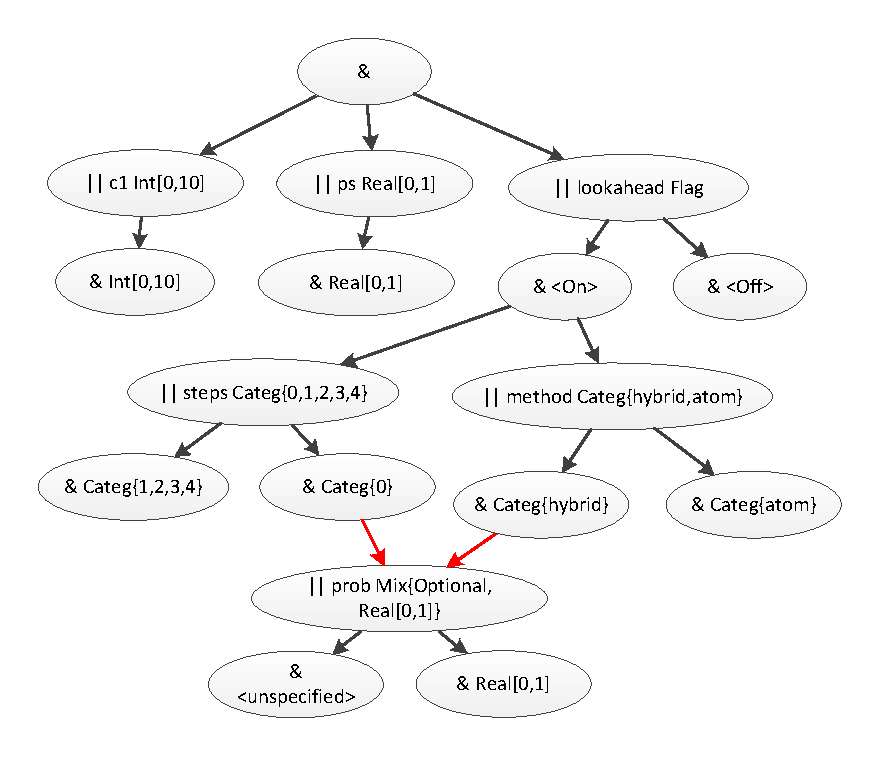
\includegraphics[width=10cm]{paramgraph.pdf}
\end{figure}

The two red edges imply the membership of the edges to the same edge group $\neq 0$. Black edges mean that the edge doesn't belong to any group.
For simplicity, the parameter references of AND-Nodes (to the same parameter as the preceeding OR-Node) are not shown in the graph.


\clearpage



\newpage
\section{Client}
\label{client}

\subsection{Introduction}
The computation is client is used to compute the jobs of experiments. Usually there have to be a lot of jobs computed to evaluate experiments
and since they are independent from each other, this task can be parallelized across many CPU cores. The computation client can be started on arbitrarily many
machines and will manage the available CPUs and start jobs from the available experiments. It connects to the central database and downloads all required resources
such as instances and solver binaries and writes back the results to the database.

\subsection{System requirements}
\label{clientSR}
\index{System requirements client}
The client is written in C/C++ and should be able to run on most Linux distributions where a MySQL C connector library is available.

Because the central storage location for all required computational ressources, experiment metadata and results is a MySQL database, the client has to be able to establish a connection to the machine that hosts the database. 
\marginlabel{TCP/IP Connections:}
This means that the machines where the client runs on have to be able to establish a TCP/IP connection
to the database machine. 

The client was mainly tested on the bwGRID\footnote{{http://www.bw-grid.de/}}, a distributed computer cluster that consists of several hundred
nodes at several physical locations at universities of Baden-W�rttemberg, Germany. Even though the machine hardware is homogenous, the network topology of bwGRID is not.
\marginlabel{Connection alternatives:}
In cases where direct network access from the computation nodes back to the database server is not possible it is usually possible to tunnel a connection
over the cluster's login node back to the database via SSH. For example running
\marginlabel{\Eexample}\begin{verbatim}
ssh -f -N -L 0.0.0.0:1234:databasehost:3306 user@databasehost
\end{verbatim}
on the login node sets up a tunnel for connections at port 1234 and forwards them to your database machine at port 3306, where MySQL listens.
The options \texttt{-f} and \texttt{-N} will let the tunnel continue to run in the background, even after logging out from the login node.
To terminate the tunnel, simply run e.g. \texttt{killall ssh} on the login node. In the client configuration (see below), you would
then specify the IP/hostname of the login node and port 1234 as the database hostname and port.

Other than that, the client has to be able to write temporary files to some location on the filesystem. This can be configured (\ref{client_command_line_arguments}) if it differs from the client binary location.

Because the client will download missing solver binaries and instances and upload results it also needs a reasonably fast network connection to the database. 
\marginlabel{Shared filesystems:}
\index{Shared filesystems}
Shared filesystems can considerably reduce the required bandwidth since every file is only downloaded once. Alternatively you can create
a package from within the GUI that contains all solver binaries and instances of an experiment. However, if you modify experiments while the client is running it will still download missing files.

\newpage
\subsection{Usage}
\subsubsection{Configuration}
\marginlabel{Configuration file:}
\index{Client configuration}
Configuration is done by some command line arguments and a simple configuration file, called ''config''. This file has to be in the \textbf{working directory} of the client at runtime.
In the configuration file you have to specify the database connection details and which hardware the client runs on. This is done by configuring so called ''grid queues'' in the GUI application.
They contain some basic information about the computation hardware such as number of CPUs per machine. The client will then use this information to run as many parallel jobs as
the grid queue information allows it on each machine where it is launched. Here is a sample configuration file:
\marginlabel{\Eexample}
\begin{verbatim}
host = database.host.foo.com
port = 3306
username = dbusername
password = dbpassword
database = dbname
gridqueue = 3
verifier = ./verifiers/SAT
\end{verbatim}
\index{Grid queue}
Note that the gridqueue value is simply the ID of the grid queue. Another (optional) configuration option is the verifier line. It tells the client if it should run a program on the output that a
solver generated. For example, if your experiments consist of attempting to solve boolean propositional logic formulas you can use a SAT verifier that tests if the solution given by a solver
is actually correct. The verifier configuration option is simply a path to an executable that the client calls with standardized parameters. See section \ref{sec:verifiers} for more information on verifiers.


Beside the configuration file there are several command line options the client accepts, please also see ''./client --help'':
\marginlabel{Command line arguments:}
\label{client_command_line_arguments}
\begin{verbatim}
-v <verbosity>:
  Integer value between 0 and 4 (from lowest to
  highest verbosity)
-l:
  If flag is set, the log output is written to a file
  instead of stdout.
-w <wait for jobs time (s)>:
  How long the client should wait for jobs after
  it didn't get any new jobs before exiting.
-i <handle workers interval ms>:
  How long the client should wait after handling
  workers and before looking for a new job.
-k:
  Whether to keep the solver and watcher output files after
  uploading to the DB. Default behaviour is to delete them.
-b <path>:
  Base path for creating temporary directories and files.
-h:
  Toggles whether the client should continue to run even
  though the CPU hardware of the grid queue is not homogenous.
-s:
  Enables simulation mode where the client will fetch and run
  jobs but won't write any results back to the database.
\end{verbatim}

Verbosity controls the amount of log output the client generates. A value of 4 is only useful for debugging purposes, a value of 0 will make the client log important messages and all errors.

If the ''l'' flag is set, log output goes to a file whose name includes the hostname and IP address of the machine the client runs on. This is done to avoid name clashes in shared filesystems typically found in computer clusters.
Otherwise log output goes to standard output.

With the ''-w'' option you can tell the client how long to wait before exiting after it didn't start any jobs. This can be useful to keep the clients running and ready to process new jobs
while you evaluate preliminary results and add new jobs or whole experiments. The wait option is also used to determine how long attempts should be made to reconnect to the database after
connection losses. The default value is 10 seconds.

The ''-i'' option controls how long the client should wait between its main processing loop iterations. If this value is low, it will look for new jobs when there are unused CPUs more frequently.
For maximum job throughput this value should be lower than the average job processing time but lower values will also put more strain on the database and increase the client's CPU usage. The default
value is 100ms which should work fine in most cases. The client will also adapt to situations where there are free CPUs but no more jobs and increase the interval internally and fall back to the configured
value once it got another job.

The ''-k'' flag tells the client that it should keep temporary job output files after a job is finished. The default behaviour is to delete them.

The ''-b'' base path option can be used to specify a directory the client can use to write temporary files to. The default value is ''.'', i.e.
the working directory at runtime.

\marginlabel{inhomogenous machines}
\attention The first client to start with a particular grid queue will write the information about the machine it runs on to the grid queue entry in the database. All following clients will then
compare their machines to the information in the grid queue and exit, unless the number of cores and the CPU model name match. With the ''-h'' option you
can override this behaviour.

\subsubsection{Launching}
After configuration you can simply run the client on your computation machines. On computer clusters there are often queuing systems that you have to use to gain access to the nodes.
On bwGRID for example, we could use the following short PBS (portable batch script) and submit (\textit{qsub scriptname}) our client to a node with 8 cores:
\begin{verbatim}
#!/bin/sh
#PBS -l walltime=10:00:00
#PBS -l nodes=1:ppn=8
cd /path/to/shared/fs/with/client/executable
./client -v0 -l -i200 -w120
\end{verbatim}
\attention You should always run the client from within its directory (i.e. cd to the directory) to avoid problems with relative paths such as the verifier path from the example configuration above.

As soon as clients start you should be able to see jobs changing their status from ''not started'' to ''running'' in the GUI's or Web frontend's job browsers.

\subsubsection{Troubleshooting}
If errors or failures occur the client will always attempt to shut down cleanly, that is stop all running jobs and set their status to ''client crashed'' and write
the last lines of its log output as ''launcher output'' to each job. This can fail when network connections fail or the client receives a SIGKILL signal causing it to exit immediately.
In case of network failures you should still be able to find useful information in the client's logfile on the local filesystem.

\subsection{Verifiers}
\label{sec:verifiers}
Verifiers are programs that the client runs after a job finishes. Verifiers are getting passed the instance of the job and the solver output as arguments and are supposed to
write a newline character followed by a (textual/ASCII) integer result code at the end of their output. The result code should convey some information about the result of
the job, for example whether the output of the solver is correct given the problem instance.
This code will be written to the database as ''result code'' while the verifier's exit code will be written as ''verifier exit code''. Any output the verifier writes to standard out will
be written as ''verifier output''. The call specification for a verifier binary looks like this:
\begin{verbatim}
./verifier_binary <path_to_instance> <path_to_solver_output>
\end{verbatim}
We provide a verifier for the SAT problem that works on CNF instances in DIMACS format and solvers that adhere to a certain output format (see the source code).
If you want to write an own verifier specific to your problem you can also use the source code as implementation example.
\attention Note that you have to make sure
that your possible result codes are specified in the \textit{ResultCodes} table in the database before running clients or there will be errors when the client tries to write results. By convention,
the web frontend and GUI application consider status codes that begin with a decimal ''1'' as correct answers.

\subsection{Experiment priorization}
\label{sec:experiment_priorization}
Sometimes it can be useful to compute several experiments in parallel but give some a higher priority than others. In order to accomplish that, experiments can be marked as inactive and individual jobs can be prioritized. Only jobs of active experiments with priority equal to or greater than 0 are considered for processing
by the client. Futhermore, experiments can be assigned a priority. The clients will then try to match the relative number of CPUs working on an experiment with its relative priority to
all other experiments that are assigned to the same grid queue. For example, if you have three experiments with priorities 100, 200 and 300 respectively the running clients will try to have 16\% of CPUs working on the first, 33\% of CPUs working on the second and 50\% of CPUs working on the third experiment.

\clearpage

\attention The client is running solely on Unix and is not distributed yet for Windows systems.

\newpage
\section{Web Frontend}
\label{web_frontend}
\upshape
\index{Web Frontend}
\subsection{Introduction}
The Web Frontend provides access to experiment information and analysis tools in a read-only manner
and accessible by a web browser.

\subsection{System requirements}
\label{wfSR}
\index{System requirements, Web Frontend}
The web frontend is implemented as Python WSGI web application and makes use of several libraries.
Since it interfaces with R to draw plots it also depends on R and a Python interface to R, which unfortunately
only works properly on Linux right now.
WSGI applications can be deployed on a variety of web servers or even run standalone on a web server that comes with the
Python standard library.
The following list contains all dependencies and prerequisites of the Web Frontend (see \ref{wf:installation} for installation instructions).
\begin{itemize}
\item Python 2.6.5 or 2.7 http://www.python.org
\item R 2.11 (language for statistical computing and graphics)
\item R package 'np' (available via R's CRAN)
\item SQLAlchemy 0.6.5 (SQL Toolkit and Object Relational Mapper)
\item mysql-python 1.2.3c1 (Python MySQL adapter)
\item Flask 0.6 (Micro Webframework)
\item Flask-WTF 0.3.3 (Flask extension for WTForms)
\item Flask-Actions 0.5.2 (Flask extension)
\item Werkzeug 0.6.2 (Webframework, Flask dependency)
\item Jinja2 2.5 (Template Engine)
\item PyLZMA 0.4.2 (Python LZMA SDK bindings)
\item rpy2 2.1.4 (Python R interface)
\item PIL 1.1.7 (Python Imaging Library)
\item Numpy 1.5.1
\item pygame 1.9 (Graphics library)
\end{itemize}

\subsection{Installation}
\label{wf:installation}
\index{Installation, Web Frontend}
To get rpy2 working the GNU linker (ld) has to be able to find libR.so. Add the folder containing
libR.so (usually /usr/lib/R/lib) to the ld config: Create a file called R.conf containing the
path in the folder /etc/ld.so.conf.d/ and run ldconfig without parameters as root to update.
Additionally, you have to install the R package 'np' which provides non-parametric statistical
methods. This package can be installed by running ''install.packages('np')'' within the R interpreter (as root).

The following installation example outlines the step that have to be taken to install the web frontend on Ubuntu 10.04
running on the Apache 2.2.14 web server. For performance reasons (e.g. query latency) the web frontend should run on the
same machine that the EDACC database runs on.
\marginlabel{\Eexample}
\begin{enumerate}
\item Install Apache and the WSGI module: \begin{verbatim}apt-get install apache2 libapache2-mod-wsgi\end{verbatim}
\item{ Copy the web frontend files to /srv/edacc\_web/, create an empty error.log file and change their ownership to the Apache user: 
\begin{verbatim}
  touch /srv/edacc_web/error.log
  chown www-data:www-data -R /srv/edacc_web
\end{verbatim}
}
\item{ Create an Apache virtual host\\
(new file at /etc/apache2/sites-available/edacc\_web)
\begin{verbatim}
<VirtualHost *:80>
  ServerAdmin email@email.com
  ServerName foo.server.com

  LimitRequestLine 51200000

  WSGIDaemonProcess edacc processes=1 threads=15
  WSGIScriptAlias / /srv/edacc_web/edacc_web.wsgi

  Alias /static/ /srv/edacc_web/edacc/static/

  <Directory /srv/edacc_web>
    WSGIProcessGroup edacc
    WSGIApplicationGroup %{GLOBAL}
    Order deny,allow
    Allow from all
  </Directory>

  <Directory /srv/edacc_web/edacc/static>
    Order allow,deny
    Allow from all
  </Directory>
</VirtualHost>
\end{verbatim}
}
\item{Install dependencies and create a virtual environment for Python libraries:
\begin{verbatim}
apt-get install python-pip python-virtualenv python-scipy
apt-get install python-pygame python-imaging
virtualenv /srv/edacc_web/env
apt-get build-dep python-mysqldb
apt-get install r-base
echo "/usr/lib/R/lib" > /etc/ld.so.conf.d/R.config
ldconfig
source /srv/edacc_web/env/bin/activate
pip install mysql-python
pip install rpy2
pip install flask flask-wtf flask-actions
pip install sqlalchemy pylzma numpy
\end{verbatim}
}
\item{Install R libraries (''R'' launches the R interpreter):
\begin{verbatim}
R
install.packages('np')
\end{verbatim}
}
\item{Create a WSGI file at /srv/edacc\_web/edacc\_web.wsgi with the following contents:
\begin{verbatim}
import site, sys, os
site.addsitedir('/srv/edacc_web/env/lib/python2.6/site-packages')
sys.path.append('/srv/edacc_web')
sys.path.append('/srv/edacc_web/edacc')
os.environ['PYTHON_EGG_CACHE'] = '/tmp'
sys.stdout = sys.stderr
from edacc.web import app as application
\end{verbatim}
}
\item Configure the web frontend by editing /srv/edacc\_web/edacc/config.py, see~\ref{wf:configuration} for details.
\item{Enable the Apache virtual host created earlier:
\begin{verbatim}
a2ensite edacc_web
service apache2 restart
\end{verbatim}
}
\item The web frontend should now be running under http://foo.server.com/
\end{enumerate}

\subsection{Configuration}
\label{wf:configuration}
\index{Configuration, Web Frontend}
All configuration is done in a Python file located at ''edacc/config.py''. The options are documented in the sample configuration
file which is included in the distribution package. Please read through the configuration options and modify those marked as important. \attention
Most importantly, you should disable debugging mode and change the secret key when making the Web Frontend
accessible from the network to avoid security problems. Logging is also quite useful to make it easier to find the cause of bugs in the application.
\marginlabel{Database configuration}At the end of the file you can configure the database connection and the list of EDACC databases that should be
made available by the Web Frontend.

\subsection{Troubleshooting}
\label{wf:troubleshooting}
\index{Troubleshooting, Web Frontend}
When there are errors or bugs and you have set up the Web Frontend under Apache as described in the installation section, Apache will display an ''Internal Server Error'' page.
If you have configured logging, the application will write tracebacks to the logging file. If you haven't set up logging, these tracebacks will end up
in Apache's error.log file.

\subsection{Features}
This section gives a short overview of the features of the Web Frontend. Most features should be self-explanatory or have some additional documentation
on the pages themself.

The Web Frontend was designed as monitoring and analysis tools of experiments that are created with the GUI application. Once you have set up some databases and added
them to the configuration file of the Web Frontend, the top level page will allow the user to select one of the databases. This leads to a page that displays
all experiments of the chosen database and some basic information about their creation date, number of solvers, instances and jobs.

\marginlabel{Experiments}
An experiment page displays further information about the experiment, such as the number of total, running and crashed jobs. If the experiment is currently
being computed, an estimation of the time of completion is displayed next to ''ETA''.

\marginlabel{Monitor progress}
Under ''Progress'' a colored bar visualizes the computation progress.
Green color corresponds to finished jobs, red to crashed jobs and orange to jobs that are currently being computed. The links following the progress bar
lead to information and analysis pages.

\index{Computation progress, Web Frontend}
\marginlabel{Job browser}
The progress page provides a job browser similar to the GUI application. It allows to sort, filter for certain words, show and hide specific columns and download
currently displayed data in CSV (comma-separated values) format\marginlabel{Export data}. Displaying more than 1000 results at once can become rather slow, since the browser's Javascript
engine has to do a lot of processing to color and format the table.

The solver configurations and instances pages show the solver configurations and instances that are part of the experiment. The instances page provides a download link
for all instance files in a tarball\marginlabel{Download instances}.
Instances are shown in a table by name, MD5 checksum and their properties (TODO reference), if there are any. The instance name links to a page that displays the 
first and last few characters of the instance file and provides a download link.

\marginlabel{View results}
\index{Results}
\index{Export results}
The result pages display the results of the jobs in various formats. ''Unsolved instances'' and ''Solved instances'' list the instances that
were not solved by any solver or solved by at least one solver respectively. ''By solver configuration'' leads to a page, where after selecting a solver configuration
that is part of the experiment a table is displayed containing all the results of the jobs of the solver configuration by instance and run number.
''By instance'' leads to a page, where after selecting an instance all results obtained on this instance are displayed by solver configuration and run number.
\marginlabel{Export results}All tables can be exported (i.e. downloaded) in CSV format.

\marginlabel{Analyse results}
\index{Analysis}
\index{Statistical tools}
\index{Visualization}
\index{Plots}
Analysis pages provide various plots of results and statistical tools such as correlation and probabilistic domination calculations. All plots can be directly saved
in PNG format as they are displayed in the browser or downloaded in PDF or EPS format\marginlabel{Export plots}\index{Export plots}. For some plots the application generates an R script which can be adjusted as
neccessary.
Most plots allow to download the underlying data in CSV format.

Some plots allow the selection of multiple instances. In this case, you can use a filter to narrow the selection of the instances listed. Please refer to the example
which is displayed next to the filter text field.

\marginlabel{Ranking of solver configurations}
\index{Ranking}
The ranking is determined by the number of successful runs but the ranking table can be sorted by any of the displayed measures.

\clearpage

\section{Monitor}

\section{Troubleshooting}



\begin{fullpage}
\stepcounter{section}
\addcontentsline{toc}{section}{\numberline {\thesection} Glossar}
\printglossary
\end{fullpage}

\printindex

\end{document}
